%!TEX program = xelatex

\documentclass[a4paper, openany, oneside]{memoir}
\usepackage[no-math]{fontspec}
\usepackage{pgfplots}
\usepackage{float}
\pgfplotsset{compat=newest}
\usepackage{commath}
\usepackage{mathtools}
\usepackage{amssymb}
\usepackage{amsthm}
\usepackage{booktabs}
\usepackage{todonotes}
\usepackage{mathtools}
\usepackage{xcolor}
\usepackage[separate-uncertainty=true, per-mode=symbol]{siunitx}
\usepackage{listings}
\usepackage[american inductor, european resistor]{circuitikz}
\usepackage{amsmath}
\usepackage{amsfonts}
\usepackage{ifxetex}
\usepackage[dutch,english]{babel}
\usepackage[backend=bibtexu,texencoding=utf8,bibencoding=utf8,style=ieee,sortlocale=en_GB,language=auto]{biblatex}
\usepackage[strict,autostyle]{csquotes}
\usepackage{import}
\usepackage{standalone}
\usepackage{bookmark,hyperref}
\usepackage{xcolor,mdframed}
\usepackage{tikz}
\usepackage{framed}
\usepackage{float}
\usepackage{tabularx}
\usepackage{graphicx,adjustbox}
\usepackage{rotating}
\usepackage{pdfpages}
\usepackage{enumitem}
\usepackage{calc}
\usepackage{pgfplots}
\usepackage{filecontents}
\usepackage{caption}
\usepackage{subcaption}
\usepackage{lettrine}

\newcolumntype{Y}{>{\raggedright\arraybackslash}X} % Left-justified text in tabularx environment

\ifxetex{} % Fonts laden in het geval dat je met Xetex compiled
    \usepackage{fontspec}
    \defaultfontfeatures{Scale=MatchLowercase, Ligatures=TeX} % To support LaTeX quoting style
    %\setromanfont{Palatino Linotype} % Tover ergens in Font mapje in root.
    \setsansfont{Avenir Next LT Pro}
    \setromanfont{Adobe Caslon Pro} % Tover ergens in Font mapje in root.
    \setmonofont{Source Code Pro}
\else % Terug val in standaard pdflatex tool chain. Geen ondersteuning voor OTT fonts
    \usepackage[T1]{fontenc}
    \usepackage[utf8]{inputenc}
\fi
\usepackage[noabbrev, capitalize]{cleveref}
\usepackage{ifthen}
\usepackage{titlesec}
\usepackage{titlecaps}

\newcommand{\references}[1]{\begin{flushright}{#1}\end{flushright}}
\renewcommand{\vec}[1]{\boldsymbol{\mathbf{#1}}}
\newcommand{\uvec}[1]{\boldsymbol{\hat{\vec{#1}}}}
\newcommand{\mat}[1]{\boldsymbol{\mathbf{#1}}}
\newcommand{\fasor}[1]{\boldsymbol{\tilde{\vec{#1}}}}
\newcommand{\cmplx}[0]{\mathrm{j}}
\renewcommand{\Re}[0]{\operatorname{Re}}
\newcommand{\Cov}{\operatorname{Cov}}
\newcommand{\Var}{\operatorname{Var}}
\newcommand{\proj}{\operatorname{proj}}
\newcommand{\Perp}{\operatorname{perp}}
\newcommand{\col}{\operatorname{col}}
\newcommand{\rect}{\operatorname{rect}}
\newcommand{\sinc}{\operatorname{sinc}}
\newcommand{\lcm}{\operatorname{lcm}}
%\newcommand{\gcd}{\operatorname{gcd}}
\newcommand{\F}{\mathcal{F}}
\newcommand{\DTFT}{\mathcal{F}_*}
\newcommand{\conj}[1]{#1^*}
\renewcommand{\mod}{\operatorname{mod}}
\newcommand{\rot}{\operatorname{rot}}
\newcommand{\vecsc}[1]{\vec{\textsc{\textbf{#1}}}}
\renewcommand{\ss}[1]{_{#1}}

% Label without linebreak breaker
\newcommand{\lab}[1]{\label{#1}\nolinebreak}

\newtheorem{definition}{Definition}
\newtheorem{theorem}{Theorem}


\DeclareSIUnit{\voltampere}{VA} %apparent power
\DeclareSIUnit{\pii}{\ensuremath{\pi}}

\hypersetup{%setup hyperlinks
    colorlinks,
    citecolor=black,
    filecolor=black,
    linkcolor=black,
    urlcolor=black
}

% Example boxes
\usepackage{fancybox}
\usepackage{framed}
\usepackage{adjustbox}
\newenvironment{simpages}%
{\AtBeginEnvironment{itemize}{\parskip=0pt\parsep=0pt\partopsep=0pt}
\def\FrameCommand{\fboxsep=.5\FrameSep\shadowbox}\MakeFramed{\FrameRestore}}%
{\endMakeFramed}

% Impulse train
\DeclareFontFamily{U}{wncy}{}
\DeclareFontShape{U}{wncy}{m}{n}{<->wncyr10}{}
\DeclareSymbolFont{mcy}{U}{wncy}{m}{n}
\DeclareMathSymbol{\Sha}{\mathord}{mcy}{"58}

\setlength{\parindent}{0pt}
\nonzeroparskip

% Block environment configuration
\newcommand{\BlockLeftMargin}{20pt}
\newcommand{\BlockLeftMarginText}{25pt}
\newcommand{\BlockLeftMarginTextSpacing}{10pt}

% Own colours
\definecolor{gray75}{gray}{0.75}

% Block environment
\newenvironment{block}[3]{%
\makebox{\hspace{-\spinemargin}%
\begin{tikzpicture}[overlay]
    \draw [thick,color=gray75] (\BlockLeftMargin, 0) -- (\paperwidth - \spinemargin, 0);
    \node at (\BlockLeftMarginText, -0.9) [align=left, text width=\spinemargin - \BlockLeftMarginText - \BlockLeftMarginTextSpacing, anchor=west, text depth=1cm] {\textbf{\textsc{#1}}\newline\textit{#3}};
\end{tikzpicture}}%
\nopagebreak\\[0.25em]\ifthenelse{\equal{#2}{}}{}{(\textit{#2}.) }\nopagebreak\nolinebreak}
{\nopagebreak\\[-0.25em]%
\makebox{\hspace{-\spinemargin}%
\begin{tikzpicture}[overlay, remember picture]
    \draw [thick,color=gray75] (\spinemargin,0) -- (\paperwidth - \spinemargin,0);
\end{tikzpicture}} \vspace{0.5em}}

% Theorem
\newcounter{blockTheoremCounter}
\crefname{blockTheoremCounter}{Theorem}{Theorems}
\Crefname{blockTheoremCounter}{Theorem}{Theorems}

\newenvironment{blockTheorem}[1][]{%
\refstepcounter{blockTheoremCounter}%
\begin{block}{theorem \theblockTheoremCounter}{#1}{}}
{\end{block}}

% Definition
\newcounter{blockDefinitionCounter}
\crefname{blockDefinitionCounter}{Definition}{Definitions}
\Crefname{blockDefinitionCounter}{Definition}{Definitions}

\newenvironment{blockDefinition}[1][]{%
\refstepcounter{blockDefinitionCounter}%
\begin{block}{definition \theblockDefinitionCounter}{#1}{}}
{\end{block}}

% Proof
\newcounter{blockProofTheoremCounter}
\crefname{blockProofTheoremCounter}{Proof}{Proofs}
\Crefname{blockProofTheoremCounter}{Proof}{Proofs}

\newenvironment{blockProofTheorem}[1]{%
\refstepcounter{blockProofTheoremCounter}%
\begin{block}{proof of \\ theorem #1}{}{}}
{\qed\end{block}}

% Detail
\newcounter{blockDetailCounter}
\crefname{blockDetailCounter}{Detail}{Details}
\Crefname{blockDetailCounter}{Detail}{Details}

\newenvironment{blockDetail}[1][]{%
\refstepcounter{blockDetailCounter}%
\begin{block}{detail \theblockDetailCounter}{#1}{}}
{\end{block}}

% Redesign chapter headings
\newcommand{\chapternumber}{\thechapter}
\newcommand{\hsp}{\hspace{20pt}}
\titleformat{\chapter}[hang]{\Huge\bfseries}{\chapternumber\hsp\textcolor{gray75}{|}\hsp}{0pt}{\Huge\bfseries}

% Remove headers
% \addtopsmarks{headings}{}{
%   \createmark{chapter}{left}{nonumber}{}{}
% }
% \pagestyle{headings} % Activate changes

% Capitalise headers in a regular way
\renewcommand*{\memUChead}[1]{\titlecap{#1}}

% \hfill for math mode
\newcommand{\pushright}[1]{\intertext{\hfill$\displaystyle #1$}}
\newcommand{\pushline}{\hskip \textwidth minus \textwidth}
\newcommand{\matlab}{\textsc{Matlab}}

\definecolor{code-grey}{HTML}{DDDDDD}
\newcommand{\lib}[1]{\textsf{#1}}
\newcommand{\file}[1]{\textsf{#1}}
\newcommand{\func}[1]{\colorbox{code-grey}{\texttt{#1}}}
\newcommand{\class}[1]{\colorbox{code-grey}{\texttt{#1}}}

% Setup actiepunten
\newenvironment{important}[1][]{%
   \begin{mdframed}[%
      backgroundcolor={red!15}, hidealllines=true,
      skipabove=0.7\baselineskip, skipbelow=0.7\baselineskip,
      splitbottomskip=2pt, splittopskip=4pt, #1]%
   \makebox[0pt]{% ignore the withd of !
      \smash{% ignor the height of !
         \fontsize{32pt}{32pt}\selectfont% make the ! bigger
         \hspace*{-19pt}% move ! to the left
         \raisebox{-2pt}{% move ! up a little
            {\color{red!70!black}\sffamily\bfseries !}% type the bold red !
         }%
      }%
   }%
}{\end{mdframed}}
\newcommand{\excl}[1]{
\begin{important}
  \textbf{#1}
\end{important}
}

\makeatletter
\newcommand\footnoteref[1]{\protected@xdef\@thefnmark{\ref{#1}}\@footnotemark}
\makeatother

% Allow page breaks in display environments
%\allowdisplaybreaks
% S unit for use in Mega Samples per second
\DeclareSIUnit\sample{S}

\newcommand{\CC}{C\nolinebreak\hspace{-.05em}\raisebox{.3ex}{ \textbf{+}}\nolinebreak\hspace{-.10em}\raisebox{.3ex}{\textbf{+}}}
\def\CC{{C\nolinebreak[4]\hspace{-.05em}\raisebox{.3ex}{\textbf{++}}}}


\newcommand{\partauthor}[1]{\gdef\@partauthor{#1}}
\renewcommand{\printparttitle}[1]{
  \parttitlefont #1\\
  \vspace{1.5cm}
  \textnormal{\Large \@partauthor}
}
\addbibresource{../../includes/bibliography.bib}

\title{Introduction}

\author{W.P. Bruinsma \and R.P. Hes \and H.J.C. Kroep \and T.C. Leliveld \and W.M. Melching \and T.A. aan de Wiel}

\raggedbottom

\begin{document}

\section{Introduction}
In this part, we develop an approach to enable high-performance spectrum sensing. More specifically, we develop techniques which are implemented in various modules of the toolkit.
spectrum sense = detectie van signal is verscheiende delen van het spctrum
- definitie

- uitleg structuur van part


\section{System overview}
- modules: \\
* Sampling techniques which allow for efficient spectrum sensing \\
* Reconstruction module which analyses the sampled signal in real-time \\
* Detection module which performs identification of the spectrum based on the output of the reconstruction algorithm \\

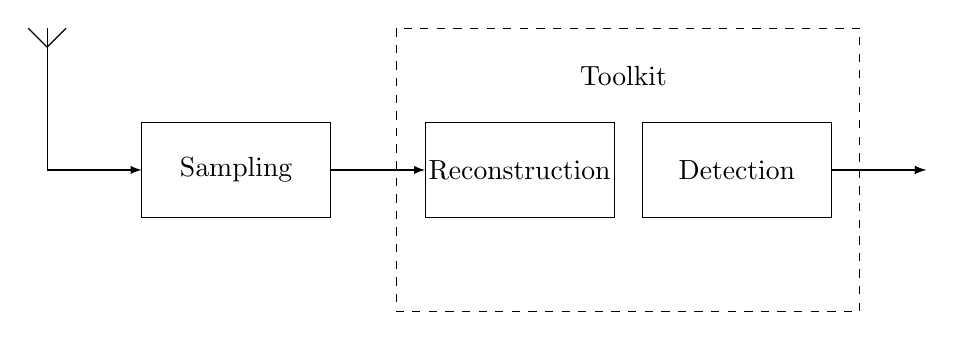
\begin{tikzpicture}[scale=1.2]

\draw  (-1,1.5) rectangle (1,0.5) node[pos=.5]{Sampling};
\draw  (2,1.5) rectangle (4,0.5) node[pos=.5]{Reconstruction};
\draw  (4.3,1.5) rectangle (6.3,0.5) node[pos=.5]{Detection};
\draw  [dashed] (1.7,2.5) rectangle (6.6,-0.5);
\node at (4.1,2) {Toolkit};

\draw [>=latex,->] (1,1) -- (2,1);
\draw [>=latex,->] (6.3,1) -- (7.3,1);
\draw [>=latex,->] (6.3,1) -- (7.3,1);
\draw [>=latex,->] (-2,1) -- (-1,1);

\draw (-2,1) -- (-2,2.5);
\draw (-1.8,2.5) -- (-2,2.3);
\draw (-2.2,2.5) -- (-2,2.3);

\end{tikzpicture}

\section{Requirements and specifications}
The requirements of our approach are as follows. The approach must enable spectrum sensing such that the application
\begin{enumerate}
    \item is able to identify at which frequencies signals are present, where signals
    \begin{enumerate}
        \item can be any signal distinct from noise and
        \item can have any reasonable signal strength;
    \end{enumerate}
    \item is able to sense any specified bandwidth and
    \item makes use of sampling techniques which are more efficient than conventional sampling techniques.
\end{enumerate}

The specifications of our approach are as follows. Identification of signals must be such that
\begin{enumerate}
    \item idenfication of signals consists of determines the set of frequencies with are occupied by signals other than noise;
    \item this identification can be done real-time;
    \item the resolution of these frequencies can be specified and
    \item the correctness of operation can be specified.
\end{enumerate}
Identification of signals should be such that
\begin{enumerate}
    \item the resolution of detection can be as high as possible and
    \item its operation can be as accurate as possible.
\end{enumerate}

The sampling techniques must be such that they allow for
\begin{enumerate}
    \item usage of a single sampling device and
    \item usage of multiple devices such that the workload can be distributed across the sampling devices.
\end{enumerate}

We will design our system according to these requirements and specifications.

% Compressive sensing is a subject that has made some important improvements in recent years. D.Ariananda and G.Leus published a paper in 2012 that proposed a new method in compressive sampling. When calculating the power spectral density of a signal, a lot of information is lost during the process. This paper exploits this fact by sampling in such a way, that only the information required to calculate the power spectral density is acquired. This allows for much less samples than Nyquist.

% Compressive sensing is an active area of research \textbf{meer}. Most algorithms are based on L1-techniques and try to recover the spectrum of the signal, and therefore assume that the signal is \emph{sparse} in the Fourier domain. Recent developments \textbf{papers van leus en ariananda hier} have shown that it is possible to reconstruct the power spectral density instead of the spectrum without the assumption of sparsity.

% This thesis targets a accessible theoretical description of the compressive sensing system implemented during 

% Main product: Extendable Toolkit for High-Performance Spectrum Sensing

% methode om high-performance te spectrum sensen



% Method which describes 

% - spectrum sensing
% - psd
% - detection
% - sampling methods
% - high-performance
% - real-time



% - uitleg hoofdstukken
% - kort systeemoverzicht + tikz

\end{document}
